\subsection{Creating the \acrshort{ast}}\label{CreatingAst}

The goal for the \acrshort{ast} was to decrease the information in the tree, while making fields on the classes for easier access to the information.
Another way could be having all the nodes connected as children on the tree, but instead of running through the trees children, and looking for specific children, the compiler instead directly access different fields on the nodes instead.
All the nodes of the \acrshort{ast} have been designed with this in mind.
For example on figure \myref{image:ASTDecl} a class structure can be seen, which consists of all the classes needed to express a declaration on the tree.
To use a previous example a declaration could be \texttt{int a = 5;}.

\begin{figure}[!ht]
\centering
 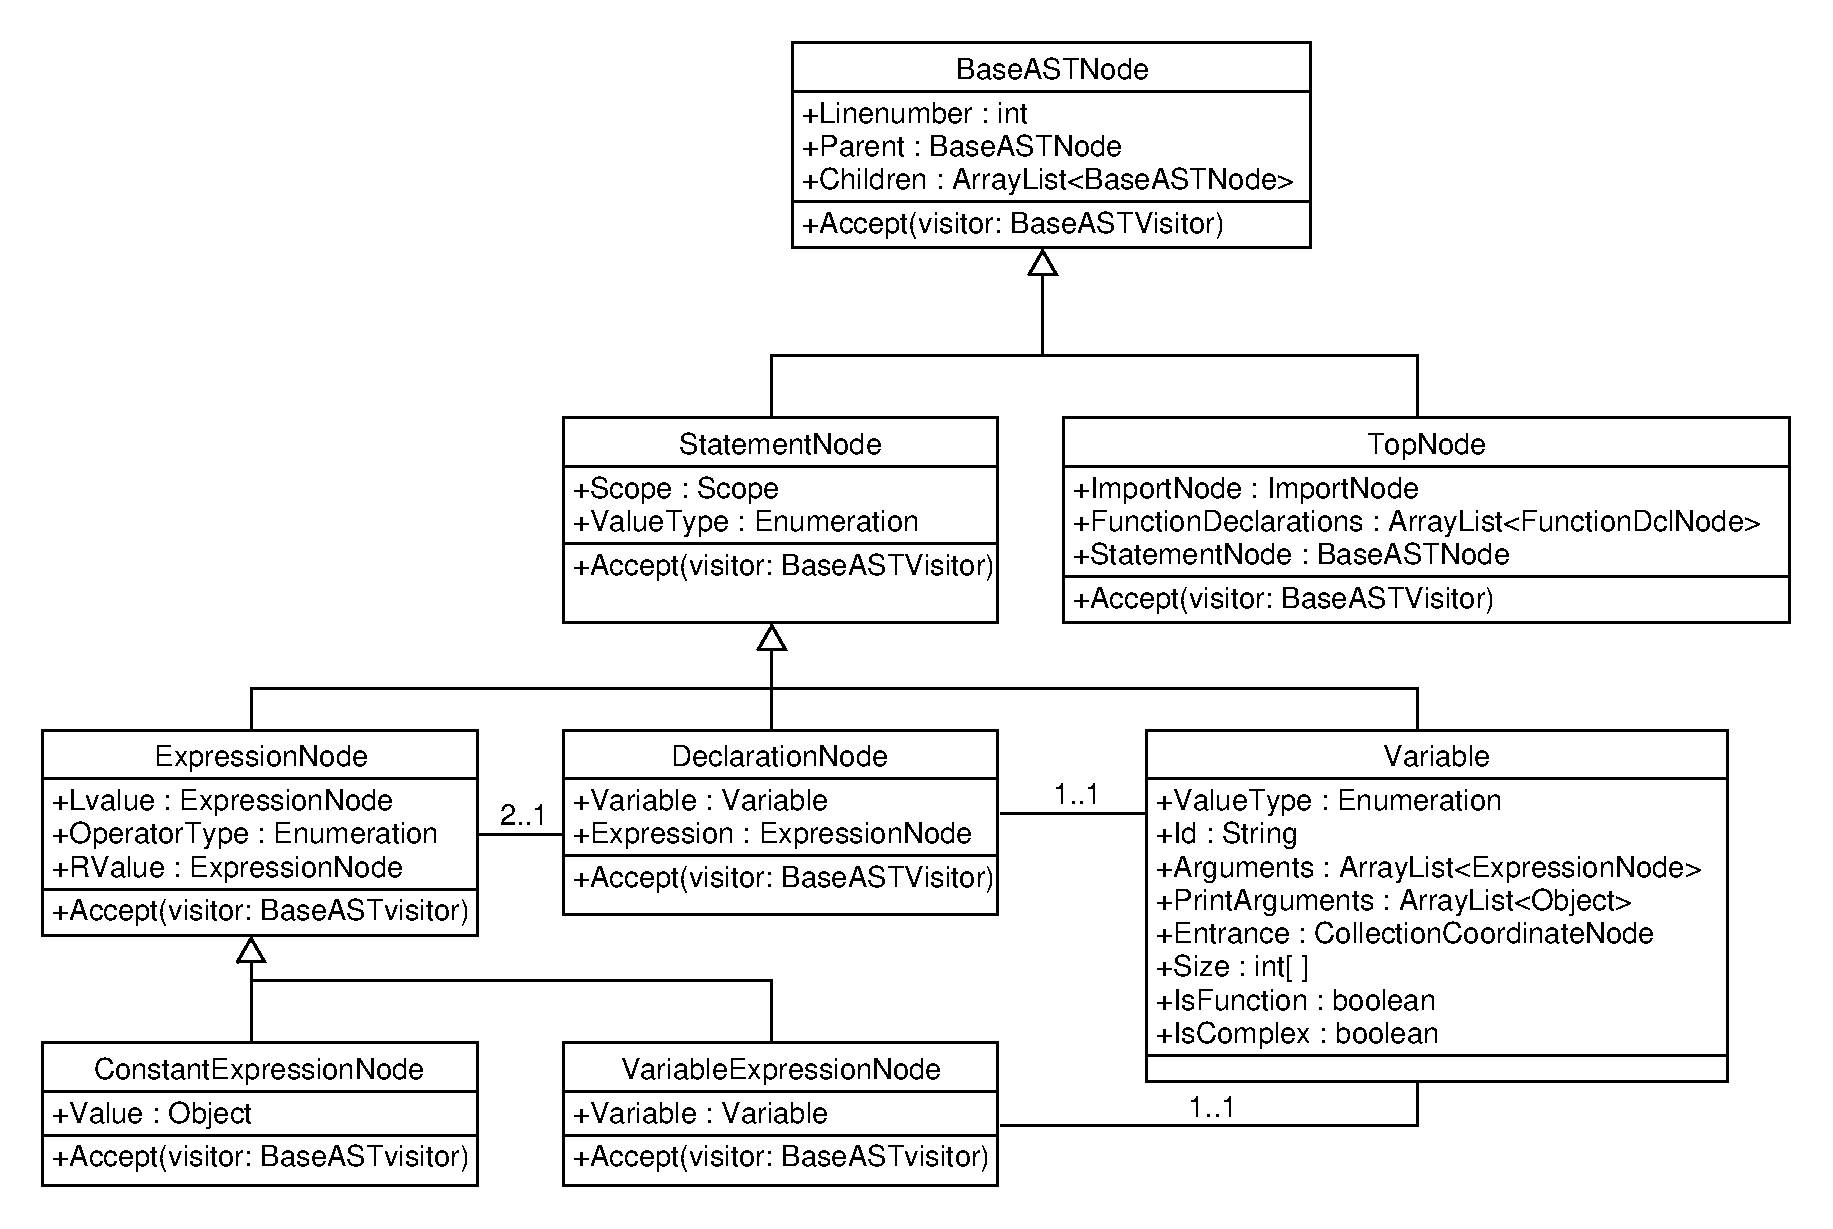
\includegraphics[width=1\textwidth]{figures/ClassDiagrams/ASTDeclarationNodeMoreInfo.pdf} % trim=4.85cm 15cm 0.85cm 1cm
\caption{A UML class diagram of the classes used for a DeclarationNode on the \acrshort{ast}.}\label{image:ASTDecl}
\vspace{-15pt}
\end{figure}

This class contains a lot of different information which is used depending on which class the instance of the \texttt{Variable} is connected to.
If \texttt{Variable} is connected to a VariableExpressionNode, the only fields used on the variable class is ValueType and Id, while the booleans IsFunction and IsComplex are set to false.
But in the example \texttt{int a = 5;} the tree structure looks like the AST on \myref{image:AST}.
If \texttt{Variable} is used when a function is on the right side of an assignment or declaration, an example being \texttt{int a = foo(5);} the fields used on \texttt{Variable} are Id, ValueType, arguments, and the boolean IsFunction is instead set to true.
The printargument field is used when the a functioncall to \texttt{Print();}is made, and entrance, size and IsComplex is used when dealing with the complex types, vectors and matrices.
\texttt{TopNode} sets the structure of a \gls{gamble} program as described in \myref{subsec:Struc}. 
The full Classdiagram can be seen on \todo{Indsæt bilag med hele klassediagrammet brugt til AST.}

